\documentclass[10pt,a4paper]{article}
\usepackage[utf8]{inputenc}
\usepackage[french]{babel}
\usepackage[T1]{fontenc}
\usepackage{graphicx}
\usepackage{listings}

\usepackage{fancyhdr}
\usepackage{vmargin}

\setlength{\parindent}{0cm}
\setlength{\parskip}{1ex plus 0.5ex minus 0.2ex}
\newcommand{\hsp}{\hspace{20pt}}
\newcommand{\HRule}{\rule{\linewidth}{0.5mm}}

\begin{document}
	\pagestyle{fancy}
	\fancyhf{}
	\rhead{SALEMI Marco, LECOCQ Alexis}
	\lhead{Pi randomness}
	\cfoot{\thepage}
	
	\begin{titlepage}
		\begin{sffamily}
			\begin{center}
				% Upper part of the page. The '~' is needed because \\
				% only works if a paragraph has started.
				
\includegraphics[scale=1.5]{images/pi.png}~\\[1.5cm]
				
				% Title
				\HRule \\[0.5cm]
				{ \huge \bfseries Pi randomness\\[0.4cm] }
				\HRule \\[1.5cm]
				
				\Large{Rapport de projet de simulation}\\[2cm]
				
				\Large{Année académique 2016-2017}\\[2cm]
				
				% Author and supervisor
				\begin{minipage}{0.4\textwidth}
					\begin{flushleft} \large
						\emph{\textbf{Auteurs :}}\\
						SALEMI Marco\\
						LECOCQ Alexis
					\end{flushleft}
				\end{minipage}
				\begin{minipage}{0.4\textwidth}
					\begin{flushright} \large
						\emph{\textbf{Directeurs :}}\\
						BUYS Alain\\
						-\\
					\end{flushright}
				\end{minipage}
				
				\vfill
				
				% Bottom of the page
				{\large \today}
				
			\end{center}
		\end{sffamily}
	\end{titlepage}
	
	\newpage
	\tableofcontents
	
	\newpage
	\section{Introduction}
	Dans le cadre du cours de simulation, nous avons été amenés à réaliser un projet afin de mettre en pratique la théorie vue au cours.
	
	Les objectifs du projet sont :
	\begin{enumerate}
		\item analyser le caractère aléatoire des décimales de pi par des tests vus au cours ;
		\item utiliser ces décimales pour construire un générateur de loi uniforme dans l'intervalle [0, 1[ ;
		\item comparer le générateur du point 2 avec celui utilisé par défaut dans Python.
	\end{enumerate}
	
	Pour ce faire, un fichier nous est fourni. Celui-ci contient les 1 000 000 premières décimales du nombre pi.
	
	Le projet doit être réalisé en python et nous avons opté pour la version 3.
	
	\newpage
	\section{Les décimales de pi}
	
	\subsection{Test de $\chi^2$}
	Le premier test consiste à étudier le nombre d'apparitions de chaque décimale. Si la séquence suit une loi uniforme, l'ensemble des décimales apparaissent exactement le même nombre de fois.
	
	\begin{figure}[h]
		\centering
		\begin{tabular}{|r|r|r|}
			\hline
			Décimales & Valeur attendue & Valeur observée\\
			\hline
			0 & 100000.0 & 99959\\
			1 & 100000.0 & 99758\\
			2 & 100000.0 & 100026\\
			3 & 100000.0 & 100229\\
			4 & 100000.0 & 100230\\
			5 & 100000.0 & 100359\\
			6 & 100000.0 & 99548\\
			7 & 100000.0 & 99800\\
			8 & 100000.0 & 99985\\
			9 & 100000.0 & 100106\\
			\hline
		\end{tabular}
		\caption{Tableau des décimales}
	\end{figure}
	
	\begin{figure}[h]
		\centering
		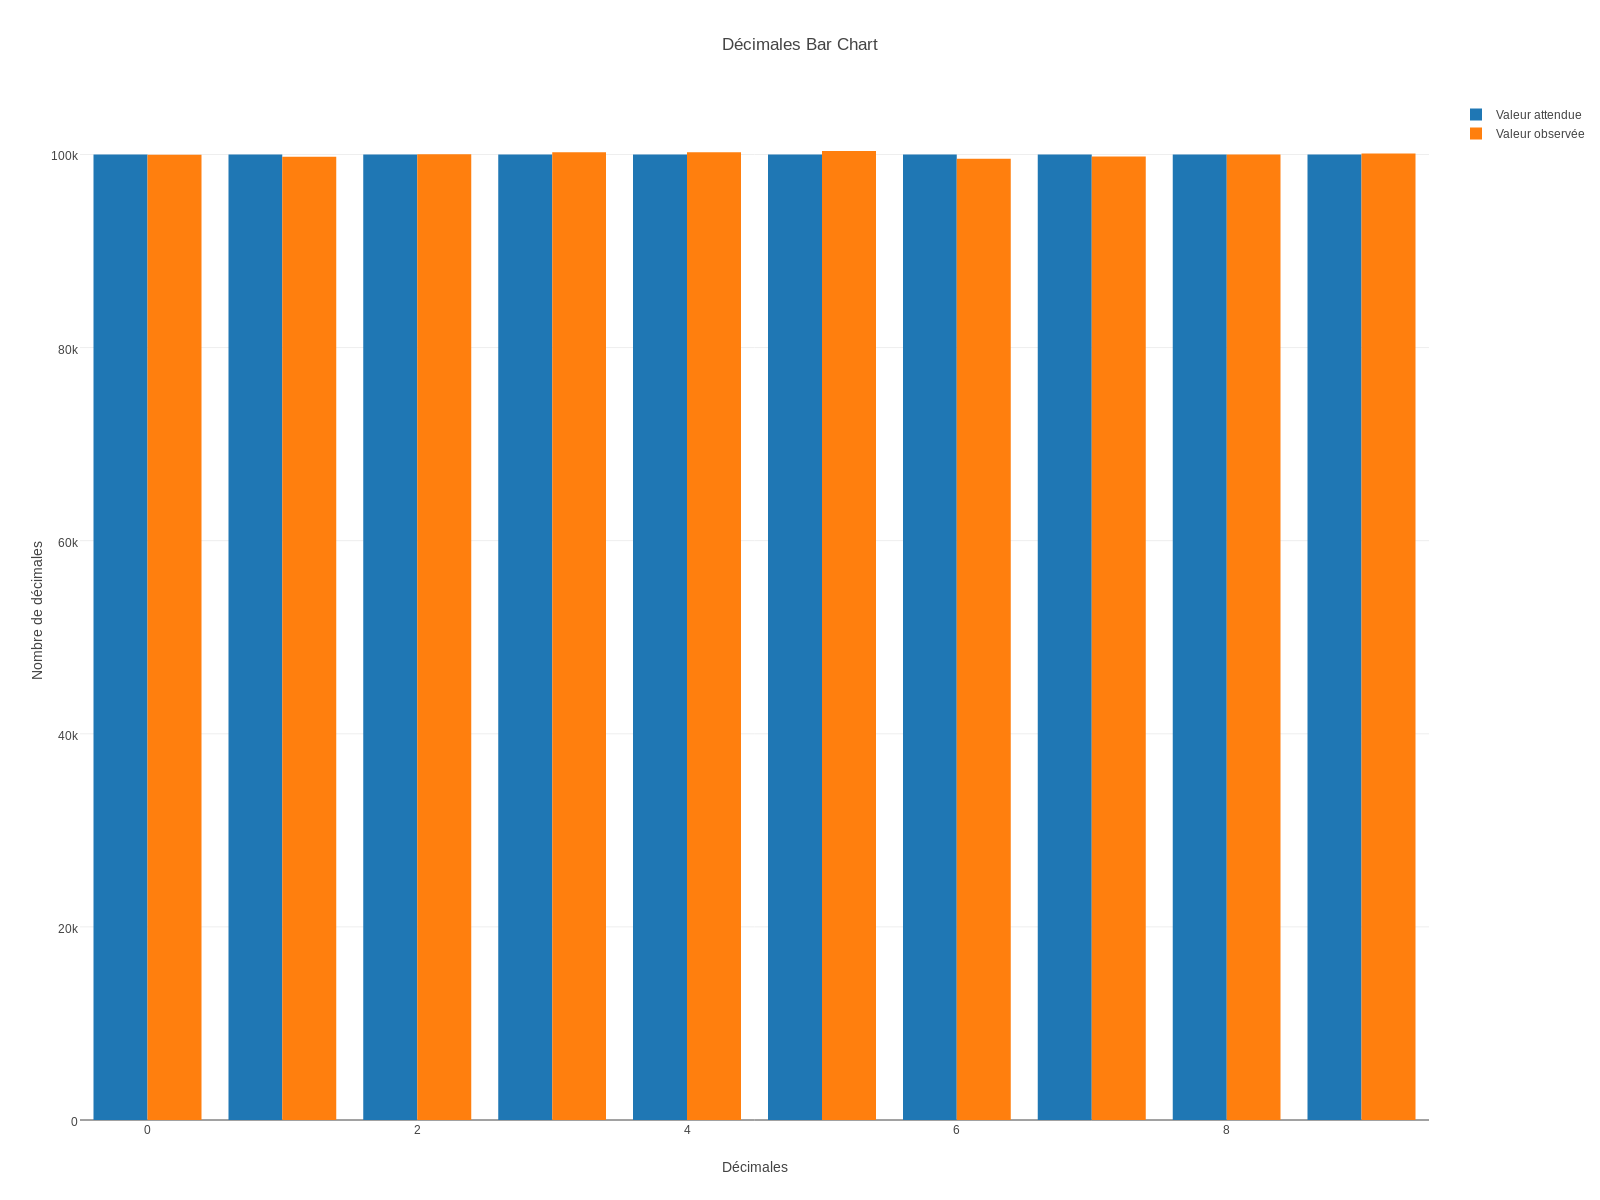
\includegraphics[scale=0.25]{../chart_images/decimales_bar_chart.png}
		\caption{Graphique des décimales}
	\end{figure}
	
	\begin{figure}[h]
		\centering
		\begin{tabular}{|r|r|r|r|}
			\hline
			$\alpha$ & Valeur & Limite & Résultat\\
			\hline
			0.001 & 5.509 & 27.877 & réussi\\
			0.01 & 5.509 & 21.666 & réussi\\
			0.05 & 5.509 & 16.919 & réussi\\
			0.1 & 5.509 & 14.684 & réussi\\
			\hline
		\end{tabular}
		\caption{Tableau du $\chi^2$}
	\end{figure}
	
	Comme nous pouvons le voir dans le tableau, le test est réussi pour tous les $\alpha$ choisis.
	
	\newpage
	\subsection{Test du poker}
	Le test du poker consiste à prendre une suite de décimales (ici 5) et calculer le nombre de décimales différentes qui composent cette suite. Si la séquence suit une loi uniforme, la probabilité d'avoir r chiffres différents dans une séquence de longueur l est :
	\[
		\frac{
			\left\{
				\begin{array}{l}
					l\\
					r\\
				\end{array}
			\right\}
			\prod_{i=10-r+1}^{10}i
		}{10^l}
	\]
	
	où $\left\{
	\begin{array}{l}
	l\\
	r\\
	\end{array}
	\right\}$ est le nombre de Stirling.
	
	\begin{figure}[h]
		\centering
		\begin{tabular}{|r|r|r|}
			\hline
			Poker & Valeur attendue & Valeur observée\\
			\hline
			1 & 20 & 13\\
			2 & 2700 & 2644\\
			3 & 36000 & 36172\\
			4 & 100800 & 100670\\
			5 & 60480 & 60501\\
			\hline
		\end{tabular}
		\caption{Tableau du Poker}
	\end{figure}
	
	\begin{figure}[h]
		\centering
		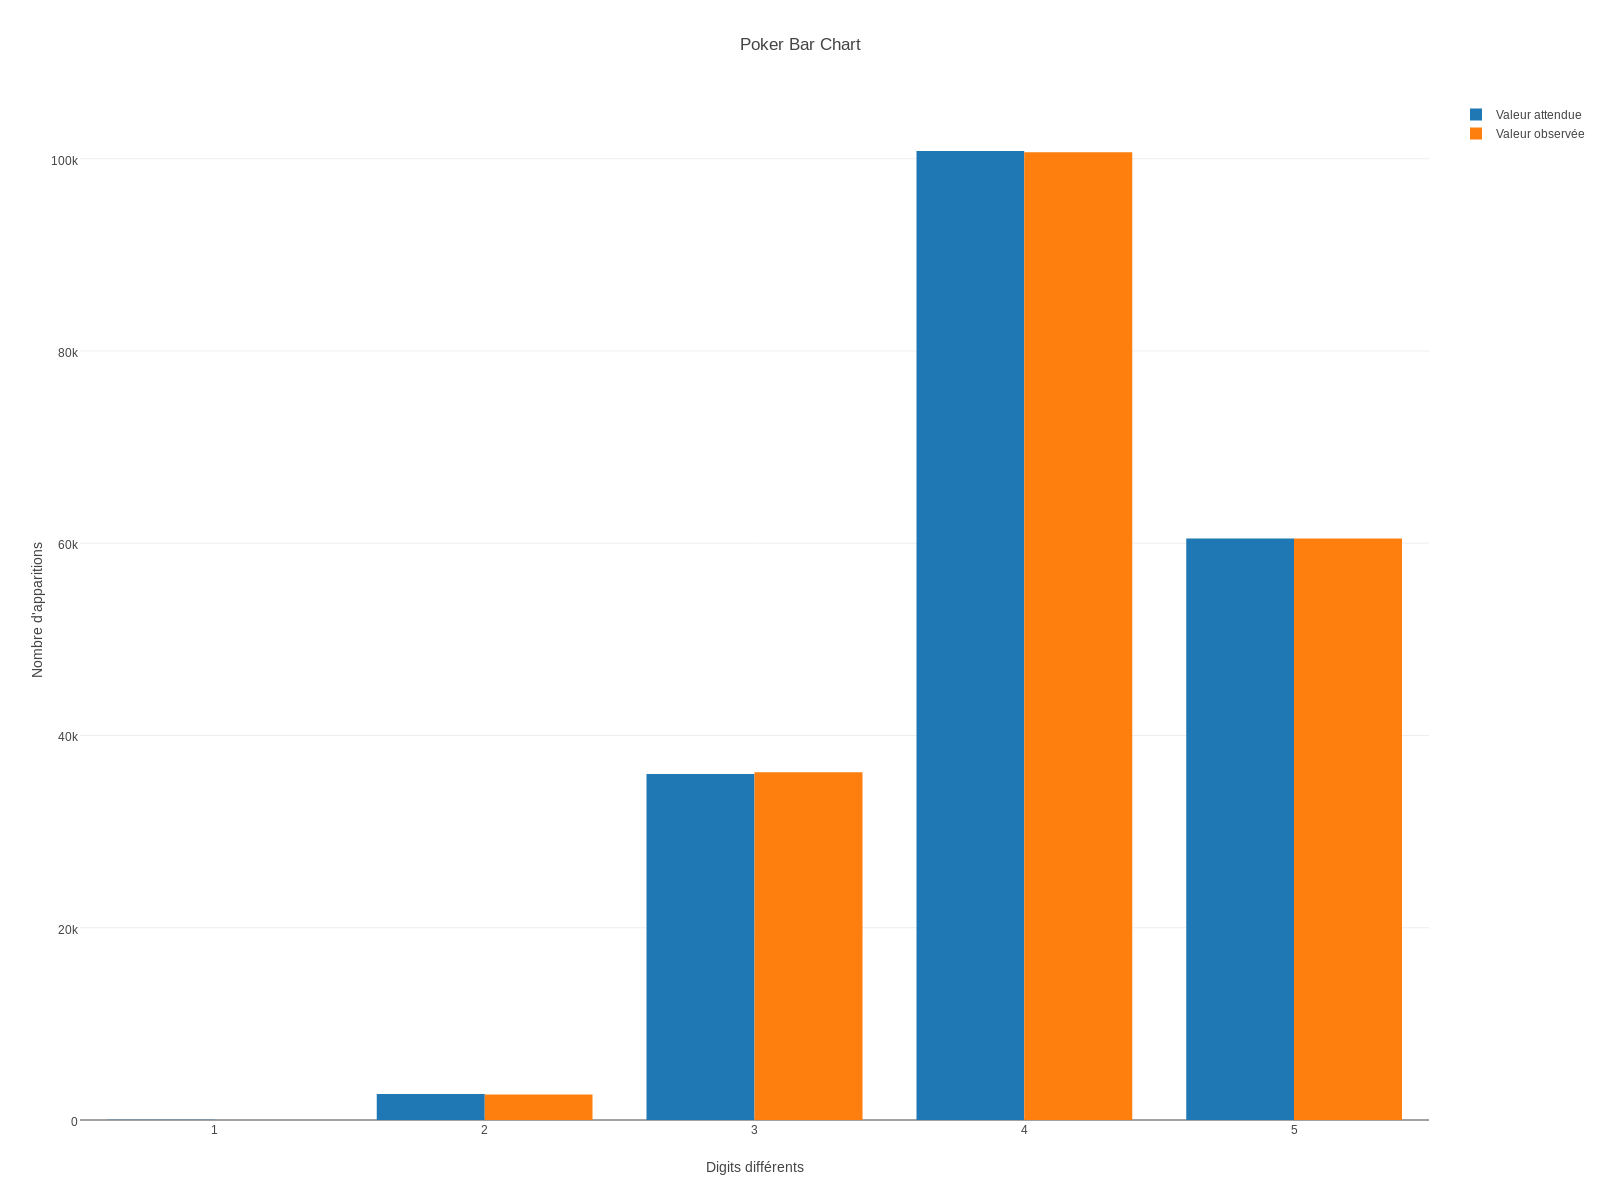
\includegraphics[scale=0.25]{../chart_images/poker_bar_chart.png}
		\caption{Graphique du Poker}
	\end{figure}
	
	\begin{figure}[h]
		\centering
		\begin{tabular}{|r|r|r|r|}
			\hline
			$\alpha$ & Valeur & Limite & Résultat\\
			\hline
			0.001 & 4.608 & 18.467 & réussi\\
			0.01 & 4.608 & 13.277 & réussi\\
			0.05 & 4.608 & 9.488 & réussi\\
			0.1 & 4.608 & 7.779 & réussi\\
			\hline
		\end{tabular}
		\caption{Tableau du $\chi^2$}
	\end{figure}
	
	Comme nous pouvons le voir dans le tableau, le test est réussi pour tous les $\alpha$ choisis.
	
	\newpage
	\subsection{Interprétation des tests}
	D'après les tests effectués ci-dessus, les décimales de pi suivent une loi uniforme.
	
	\newpage
	\section{Générateur de loi uniforme}
	Notre générateur est très simple et suit ces étapes :
	\begin{enumerate}
		\item lecture des 15 premiers chiffres à l'emplacement actuel comme un nombre ;
		\item division de ce nombre par $10^{15}$ afin d'obtenir un nombre dans l'intervalle [0, 1[.
	\end{enumerate}
	Quand nous arrivons à la fin du fichier, nous revenons au début pour que le générateur ne s'arrête jamais.
	
	Afin que le générateur ne commence pas toujours la séquence au même emplacement, nous choisissons l'emplacement de départ en fonction d'un timestamp. Ce timestamp représente le nombre de millisecondes écoulées depuis le 1er janvier 1970 UTC.
	
	La période de ce générateur est de 200 000. En effet, si le premier nombre est extrait du début du fichier, après 66 667 ($\lceil\frac{1 000 000}{15}\rceil$) mouvements de 15 caractères, nous nous retrouvons à 5 caractères plus loin qu'initialement. Après 66 667 mouvements, nous nous retrouvons 10 caractères plus loin. Si après 66 667 mouvements, nous aurions été 15 cratères plus loin, après 66 666 mouvements, nous revenons au point initial. Nous avons donc lu 3*66 666 +2 nombres aléatoires avant de relire le premier.
	
	\newpage
	\section{Comparaison avec le générateur par défaut de Python}
	Nous allons effectuer les tests vu au cours à la fois sur notre générateur et sur le générateur de python afin d'obtenir un indice de comparaison.
	
	\subsection{Test de $\chi^2$}
	
	\newpage
	\subsection{Interprétation des tests}
	Malgré la simplicité de notre générateur, celui-ci donne de très bons résultats. Cela peut s'expliquer par le fait que nous n'avons effectué nos tests que sur les 1 000 000 premiers nombres aléatoires. En effet, la période de notre générateur est de 200 000 alors que la période du Mersenne Twister (utilisé par défaut dans python) est de $2^{19937}$.
	
	D'après les tests effectués ci-dessus, ... % TODO
	
	\newpage
	\section{Conclusion}
	Nous avons bien réalisé les objectifs fixés dans l'introduction, à savoir analyser le caractère aléatoire des décimales de pi, construire un générateur uniforme et le comparer au générateur par défaut de Python.
	
	Nous avons ainsi eu l'occasion de mettre en pratique et d'approfondir les concepts vus au cours théorique notamment les test de $\chi^2$, le test du poker, le test de Kolmogorov-Smirnov, ...
	% TODO complete tests
	
	Nous tenons à remercier le titulaire BUYS Alain pour le dévouement dont il a fait preuve cette année.
	
\end{document}